
% !TEX root = ../presentation.tex



\subsection{Overview}

\begin{frame}[plain]%{Project overview}
    %\ifOnlyNotes\else
    \begin{textblock*}{0.98\paperwidth}(0.2cm,0.6cm)
        \ifOnlyNotes\else
        \foreach \x in {1,...,7}{
                \only<\x>{\adjincludegraphics%
                [width=0.98\paperwidth,trim={{0.08\width} {0.4\height} {0.08\width} {0.1\height}},clip]%
                {figs/Page\x.png}}
        }%
        \fi
    \end{textblock*}
    % \uiobigimage{?}

% *************************************
% NOTES *******************************
\begin{notes}[7]
    \nnote{1}{}
    \nnote{2}{}
    \nnote{3}{}
    \nnote{4}{\textcolor{O1}{Which will be addressed in the analysis section}}
    \nnote{5}{\dots}
    \nnote{6}{Backing up a bit; mention that curvature affects both directly and by propagation}
    \nnote{7}{These arrows are not ``rigorous;'' but they emphasise the (non-linear) thesis methodological steps}
\end{notes}
% *************************************
\end{frame}







\begin{frame}{\only<1-2>{Toy scenario}\only<3>{\textcolor{B1}{Alternative} toy scenario}}
    % {
    % \newcommand{\nSpecial}[1]{\only<1>{#1}}
    % \newcommand{\nGeneral}[1]{\only<2->{\textcolor{B1}{#1}}}
    % \newcommand{\specialgeneral}[2]{\only<1>{#1}\only<2>{\textcolor{B1}{#2}}}
    % ---
       
    
    \uncover<1->{\small
    The (\only<1-2>{\(3\)}\only<3>{\textcolor{B1}{\(N\)}}+1)%(\specialgeneral{3}{N}+1)
    -dimensional spacetime $\mathscr{M}$ is described by the metric $g\_{\mu\nu}=a^2\eta\_{\mu\nu}$ and \only<1-2>{\textbf{Cartesian comoving coordinates}}\only<3>{\textcolor{B1}{arbitrary coordinates}} $x\^{\mu}$. %
    % We impose \textbf{Cartesian comoving coordinates} in a manifold $\mathscr{M}$ 
    We consider a \only<1-2>{\textbf{matter-dominated}}\only<3>{\textcolor{B1}{[perfect fluid]-dominated}} 
    ({\(a\sim \tau^\alpha\), \( \alpha\only<1-2>{=2}\only<3>{\in \Real} \)}) 
    universe in which a \only<1-2>{\textbf{symmetron}}\only<3>{\textcolor{B1}{first-order}} phase transition takes place at scale factor $a=a_\ast$. This induces the formation of a \only<1-2>{\textbf{domain wall}}\only<3>{\textcolor{B1}{topological defect}} with (unperturbed) \only<1-2>{planar}\only<3>{simple} structure, oriented perpendicular to the \only<1-2>{$z$-axis}\only<3>{\textcolor{B1}{unit-normal $n\^\mu$}}.
    }
    % A ``planar'' domain wall is formed, with position $X\^\mu = (\tau, x, y, z_0+ \epsilon(\tau,x,y))$.
    % inducing a domain-wall formation
    % \bigskip
    % \comment{Figure?}
    % }%

    \medskip
    \uncover<2->{%
        \small
        The defect is represented by the hypersurface $\varSigma$ that splits the ambient spacetime into vacuum domains $\mathscr{M}_\pm$ with energies $\only<3>{\mathcolor{B1}}{v_\pm}\only<1-2>{=v_+}$. We let $\gamma\_{ab}$ be the induced metric on the submanifold and impose the coordinate system $\xi\^a$, where \only<1-2>{$a=0,1,2$}\only<3>{$a=0,1, \dots, N-1$}. 
        When $n\^\mu=\Krondelta{^\mu_z}$, the hypersurface's energy density\only<1-2>{---the \textbf{surface tension}---\!} is
        \begin{equation}
            \only<1-2>{\sigma}\only<3>{\mathcal{E}}=-\integ{z}[\varSigma] \sqrt{g\_{zz}} T\iud{0}{0}.
        \end{equation}
    }




% *************************************
% NOTES *******************************
\begin{notes}[3]
    \nnote{1}{\begin{itemize}
        \item Introduce terminology, specify example.
        \item We discuss only the following specific scenario, to keep the number of free parameters to a minimum.
    \end{itemize}
        % {~* Introduce terminology, specify example.}
        % {~* We discuss only the following specific scenario, to keep the number of free parameters to a minimum.}
    }
    \nnote{2}{}
    \nnote{3}{\textcolor{O1}{We discuss to various depths the possibility of generalising these parameters of the framework.}}
\end{notes}
% *************************************
\end{frame}


% \begin{frame}%{Toy scenario, continued}

%     \small
%     The induced metric is
%     \begin{equation}
%         \gamma\_{ab} \equiv a^2 \hat{\gamma}\_{ab} = a^2 \eta\_{\mu\nu}\partial\_a X\^\mu \partial\_b X\^\nu
%     \end{equation}
%     where $X\^\mu$ %=(\tau, x, y, z_0+\epsilon)$ 
%     is the wall's position. Choose $\xi\^a= \Krondelta{^{a}_{\mu}}x\^\mu$ and let $\epsilon(\xi\^a)$ be a first-order displacement to the wall's $z$-coordinate, i.e.
%     \begin{equation}
%         X\^\mu = \Krondelta{^{\mu}_{a}} \xi\^a + \Krondelta{^{\mu}_{z}} \pclosed{z_0 + \epsilon} = (\tau, x, y, z_0+\epsilon).
%     \end{equation}
%     \medskip

%     We have $a=a_\ast {(\tau/\tau_\ast)}^\alpha = a_\ast {(\tau/\tau_\ast)}^2$ and let a dot signify conformal time derivative; $\dot{} \equiv \diff/{\diff \tau}$. %\dv*{}{\tau}$.


% % *************************************
% % NOTES *******************************
% \begin{notes}[1]
%     \nnote{1}{}
% \end{notes}
% % *************************************
% \end{frame}









% |||||||||||||||||||||||||||||||||
% |||||| DW <-> hypersurface ||||||
% |||||||||||||||||||||||||||||||||

\subsection{DW \(\leftrightarrow\) hypersurface}

\begin{frame}{DW $\leftrightarrow$ hypersurface}
    \only<1>{
        \centering
        \bigskip
        \fcolorbox{B2}{B2}{\textcolor{white}{\huge\textbf{First approach}}}
    }
    % \only<2->{}
    \only<2->{
    \textcolor<3->{uiogrey}{Wall positioned at $X\^\mu = \Krondelta{^{\mu}_{a}} \xi\^a + \Krondelta{^{\mu}_{z}} \pclosed{z_0 + \epsilon} = (\tau, x, y, z_0+\epsilon)$.} %

    \only<2>{
        \ifOnlyNotes\else
        \begin{textblock*}{\textwidth}(1cm,3cm)
            % \fcolorbox{paletaupe}{white}{\parbox{\textwidth}
            {\small\color{paletaupe}{
            The induced metric is
            \begin{equation*}
                \gamma\_{ab} \equiv a^2 \hat{\gamma}\_{ab} = a^2 \eta\_{\mu\nu}\partial\_a X\^\mu \partial\_b X\^\nu
            \end{equation*}
            and $\epsilon(\xi\^a)$ is a first-order displacement to the wall's $z$-coordinate.
            
            \medskip
            We have $a=a_\ast {(\tau/\tau_\ast)}^\alpha = a_\ast {(\tau/\tau_\ast)}^2$ and let a dot signify conformal time derivative; $\dot{f} \equiv \diff f/{\diff \tau}$. %\dv*{}{\tau}$.
            }}
            % }
        \end{textblock*}
        \fi
    }

    \uncover<3->{
    \medskip
    The \newconcept{Nambu--Goto action} %
    \uncover<4->{\textcolor{G2}{with time-dependent surface tension}}
    \begin{equation}
        S\nped{NG} = - \invisible<4>{\sigma} \integ[3]{\xi \sqrt{-\gamma}}[\varSigma] \uncover<4>{\mathcolor{G2}{\sigma}}  = 
        - \uncover<3>{\sigma}\integ[3]{\xi \sqrt{-\hat{\gamma}}}[\varSigma] a^3 \uncover<4>{\mathcolor{G2}{\sigma}}
    \end{equation}
    gives the equation of motion (e.o.m.)%\note[item]<2->{under small variations}
    \begin{equation}
        \ddot{\epsilon }+ 
        {\mathcal{D}(\tau)}
        \dot{\epsilon }- \bclosed{\partial_x^2 + \partial_y^2} \epsilon = 0 
    \end{equation}
    %
    where $\mathcal{D}(\tau) = 3 \dot{a}/a\only<3>{.} \uncover<4>{\mathcolor{G2}{+\dot{\sigma}/{\sigma}}.}$
    }}

% *************************************
% NOTES *******************************
\begin{notes}[4][1st approach]
    \nnote{1}{Submanifold of two spatial dims (infinitely thin wall)}
    \itnote{2}{
        \item first-order pert. -->> induced metric
        \item moving on \dots
    }
    \itnote{3}{
        \item \textcolor{O1}{Energy times the area swept out by the worldsheet}
        \item under small variations
        \item not the first ones to get here (power-law expansion)
    }
    \nnote{4}{Modification, inspo from symmetron}
\end{notes}
% *************************************
\end{frame}










\begin{frame}{Domain-wall dynamics}%{DW $\leftrightarrow$ hypersurface}
    Separable equation $\leadsto$ Solutions $\epsilon(\tau, x, y)\sim \sum_p \varepsilon(\tau) \cdot \sppt(x,y)$, where
    \begin{subequations}
        \begin{align}
            \ddot{\varepsilon} + \mathcal{D} \dot{\varepsilon} &=- p^2 \varepsilon,  \\
            \bclosed{\partial_x^2 + \partial_y^2} \sppt &= -p^2 \sppt,
        \end{align}
    \end{subequations}
    are the solutions with eigenvalue $-p^2$. 
    
    
    % The solution to 
    % Separabel eq etc. 

    \medskip
    \uncover<2->{
        Introduce $s\equiv \tau/\tau_\ast$ and $\omega \equiv p\tau_\ast$ such that ($\sigma' \alt<2>{=}{\mathcolor{G2}{\neq}} 0$)
        \begin{equation}
            \varepsilon'' + \pclosed{\only<2>{6/s}\only<3>{\mathcolor{G2}{\tau_\ast \mathcal{D}}}}\varepsilon' + \omega^2 \varepsilon = 0.
        \end{equation}
        General solution: \only<2>{$\varepsilon(s)  = s^{\nu}\Cylindrical[\nu](\omega s)$; $\nu = (1-3\alpha)/2 = -5/2$}\only<3>{$\varepsilon(s)= \mathcolor{G2}{\boldsymbol{?}}$}.
    }

    % \uncover<3->{
    %     \paragraph{Constant surface tension.} $\varepsilon = s^{\nu}\Cylindrical[\nu](\omega s)$, $\nu = (1-3\alpha)/2 = -5/2$
    % }

% *************************************
% NOTES *******************************
\begin{notes}[3]
    \nnote{1}{Expand into eigenvalue solutions}
    \nnote{2}{Resembles a damped harm. oscillator}
    \nnote{3}{}
\end{notes}
% *************************************

\end{frame}



\begin{frame}[t]{Symmetron solution}
    \smallskip
    % Symmetron domain walls have $\sigma = \sigma_\infty \sqrt{1-\upsilon}^3$ where $\upsilon\equiv\pclosed*{a_\ast/a}^3=s^{\only<1>{-3\alpha}\only<2->{-6}}$, and this gives
    % \begin{equation}
    %     \varepsilon'' + \pclosed{ \frac{\only<1>{3\alpha}\only<2->{6}}{s} + 2d(s)} \varepsilon' + \omega^2 \varepsilon = 0; \quad d(s) \triangleq \only<1>{\frac{9 \alpha}{4s(s^{3\alpha} -1)}}\only<2->{\frac{9}{2s(s^{6} -1)}}.
    %     % \only<2->{\varepsilon'' + \pclosed{ \frac{6}{s} + 2d(s)} \varepsilon' + \omega^2 \varepsilon = 0; \quad d(s) \triangleq \frac{9}{2s(s^{6} -1)}.}
    % \end{equation}
    Symmetron domain walls have $\sigma = \sigma_\infty \sqrt{1-\upsilon}^3$ where $\upsilon\equiv\pclosed*{a_\ast/a}^3=s^{-6}$, and this gives
    \begin{equation}
        \varepsilon'' + \pclosed{ \frac{6}{s} + 2d(s)} \varepsilon' + \omega^2 \varepsilon = 0; \quad d(s) \triangleq \frac{9}{2s(s^{6} -1)}.
    \end{equation}

    \smallskip
    \uncover<1->{Initial conditions (ICs): $\varepsilon(s=1)=\epsast$ and $\varepsilon'(s=1)=0$.}
    \uncover<2->{Solve in two regimes and sow together at $s=s\ped{sow}$,
    % \only<4>{~\Here{$s\ped{sow}=1+\omega^{-1}$}}
    such that 
    \uncover<3>{$\mathcolor{k02}{\varepsilon}= \Heaviside(s\ped{sow}-s)\mathcolor{B1}{\varepsilon\ap{\tiny (I)}} + \Heaviside(s-s\ped{sow})  \mathcolor{G1}{\varepsilon\ap{\tiny (II)}}; $}
    }%
    \only<2>{
        \only<1-2>{
        \begin{equation}
            \mathcolor{k02}{\varepsilon}(s) = 
            % \begin{cases}
            %     \varepsilon\ap{\tiny (I)}(s) &\text{for } s\sim 1,\\
            %     \varepsilon\ap{\tiny (II)}(s) &\text{for } s\gg 1,
            % \end{cases}  
            % \to          
            \begin{cases}
                \mathcolor{B1}{\varepsilon\ap{\tiny (I)}}(s) &\text{if } s\leq s\ped{sow},\\
                \mathcolor{G1}{\varepsilon\ap{\tiny (II)}}(s) &\text{if } s\geq s\ped{sow}.
            \end{cases}
        \end{equation}
    }}
    %
    \only<3>{
        \begin{equation}
            \begin{split}
                \mathcolor{B1}{\varepsilon\ap{\tiny (I)}}/\epsast&\simeq 1 - \omega^2 {(s-1)}^2/5 + \omega^2 {(s-1)}^3/35 ,\\
                \mathcolor{G1}{\varepsilon\ap{\tiny (II)}}/\epsast &\simeq \mathcolor{R1}{\zeta}(s) \times s^{9/2} (s^6 - 1)^{-3/4}; \quad \mathcolor{R1}{\zeta} (s)\simeq \underbrace{s^{\nu} \Cylindrical[\nu](\omega s)}_{\text{\textcolor{O3}{``naive''}}}, \nu=-5/2.
            \end{split}
        \end{equation}
        % Here: \fcolorbox{black}{uioyellow}{$s\ped{sow}$}$=1+\omega^{-1}$.
    }

% *************************************
% NOTES *******************************
\begin{notes}[3]
    \nnote{1}{MD + ICs, \textcolor{O1}{Neat!} (possible for any $\alpha$)}
    \itnote{2}{
        \item Will not go into detail about how this equation was solved.
        \item Comment about singularity?
        \item In a region where they overlap. %\textbf{Here:} $s\ped{sow}=1+\omega^{-1}$}
    }
    \nnote{4}{}
\end{notes}
% *************************************
\end{frame}




\uiofullpageimage{../../figs/Methodology/demo_analytical_epsilon.pdf}%
\notesImage[$\zeta$ and ``naive'' are same general solution with different initial conditions 
    * Surface-tension evolution gives ]




% \begin{frame}[t]{Stress--energy tensor \comment{Remove?}}
%     \smallskip
%     Variation of the Nambu--Goto action $S\nped{NG}$ gives
%     \begin{equation}
%         T\^{\mu\nu}\rvert\nped{NG} = \frac{\sigma \Diracdelta(r)}{\sqrt{-g}\sqrt{-\gamma}} \Fdv{\gamma}{g\_{\mu\nu}} = \frac{\sigma \Diracdelta(r)}{a^3} \Fdv{\hat{\gamma}}{\eta\_{\mu\nu}},
%     \end{equation}
%     where $r\triangleq z-(z_0 + \epsilon)$. \uncover<2->{To first order in $\epsilon$, this gives
%     \begin{equation}
%         \begin{split}
%             W\_{ab}&=- a \sigma\cdot \Diracdelta(r) \cdot \eta\_{ab}, \\
%             W\_{iz}&=- a \sigma\cdot \Diracdelta(r) \cdot \partial\_{i}\epsilon.
%         \end{split}
%     \end{equation}
%     }

%     \medskip
%     \only<3>{\SideNote{Thick walls.}{
%         \( \Diracdelta(r) \to  \varPhi_l(r)\equiv [2\ppi l^2]^{-1/2} \exp{- r^2 / {(2l^2)} } \), $l\sim$ wall thickness.
%     }}

%     \only<4->{For simplicity, let $\epsilon=\varepsilon(\tau) \sppt(y) = \varepsilon(\tau) \sin(py)$.} 


% % *************************************
% % NOTES *******************************
% \begin{notes}[4]
%     \nnote{1}{}
% \end{notes}
% % *************************************
% \end{frame}






\begin{frame}{Gravitational waves}
    % The linearised Einstein equations in the TT gauge reduce to $\sq h_P= -16\piGN \pi_P$, which is solved in Fourier space through Green's functions:
    
    \begin{textblock*}{\paperwidth-0.3cm}(0.0cm,0.3cm)
        \begin{flushright}
            \ifOnlyNotes\else
            \fcolorbox{B3}{B3}{\footnotesize\color{white}{
            \(\Fdv*{S\nped{NG}}{g\_{\mu\nu}} \longrightarrow  T\^{\mu\nu} \longrightarrow  \tilde{T}\^{\mu\nu} \longrightarrow \tilde{\pi}\_{ij}  \longrightarrow \tilde{\pi}_P \longrightarrow \tilde{h}_P \)
            }}
            \fi
        \end{flushright}
    \end{textblock*}

    % \medskip
    The e.o.m. for GWs, \(\sq h_P = - 16 \piGN\pi_P\), %$\ah \equiv a h$ 
    % \begin{equation}
    %     \sq h_P = - 16 \piGN\pi_P; 
    % \end{equation}
    is solved in Fourier space through Green's functions:
    \begin{equation}
        a\tilde{h}_P(\tau, \vec{k}) \propto k^{-2} \integ{\hat{\tau}}[\tau_\ast][\tau] G(k\tau, k\hat{\tau}) a^3(\hat{\tau}) \tilde{\pi}_P  %\tilde{T}_{ij}^{\text{TT}}
        (\hat{\tau}, \vec{k}); \quad P=+,\times,
    \end{equation}
    where $G(u,v) = \RiccatiBessel[1](u)\RiccatiNeumann[1](v)-\RiccatiNeumann[1](u)\RiccatiBessel[1](v)$.\footnote<1>[5]{Riccati--Bessel functions: \( \RiccatiBessel[n](x) =+  x\sphBessel[n](x) \), \( \RiccatiNeumann[n](x) =- x\sphNeumann[n](x) \)} %
    % and $P=+,\times$. \par
    % We %defined $\ah \equiv ah $ and 
    \par
    \medskip
    {\small\color{paletaupe}{We use ICs $\tilde{h}(\tau_\ast, \vec{k})= \dot{\tilde{h}}(\tau_\ast, \vec{k})=0$.}}


% *************************************
% NOTES *******************************
\begin{notes}[1]
    \nnote{1}{Vary NG action $\to$ Analytical expression for SE tensor (with simple function)}
\end{notes}
% *************************************
\end{frame}


\begin{frame}[b]
    With \fcolorbox{R2}{white}{$\epsilon=\varepsilon(\tau)\sin(py)$,} only \emph{monochromatic plus-polarised GWs} are produced. 

    \medskip
    For $\ell \equiv k_y/p \in \Integer$ and $\vartheta \equiv \arctan(k_y/k_z)\in [0, 2\ppi)$, we have
    \begin{equation}
        a\tilde{\pi}_+ \propto  \sigma \cos^2{\vartheta}\cdot  \Bessel[-\ell] (\ell \tan{\vartheta} \cdot p\varepsilon).
    \end{equation}
    Finally,
    \begin{align}
        % \begin{split}
            a\tilde{h}_+\only<3>{^{\text{\tiny{NG}},\phi}} &\propto \mathcolor{black}{\integ{\hat{\tau}}[\tau_\ast][\tau] G(k\tau, k\hat{\tau}) \hat{\tau}^4 \sqrt{1-\pclosed{\tau_\ast/\hat{\tau}}^6}^{3} \Bessel[\ell] (\ell \tan{\vartheta} \cdot p\varepsilon\only<3>{^{\text{\tiny{NG}},\phi}}(\hat{\tau}))}.\\
            \uncover<2>{
            % &\sim \text{Bessel} \cross \int \text{Bessel} \cross \text{Bessel}(\text{Bessel})
            \mathcolor{G3}{
            &\sim \text{<<~}\Cylindrical[3/2](k\tau) \cross \integ{\hat{\tau}}  \Cylindrical[3/2](k\hat{\tau}) \cross \Bessel[\ell]\bclosed{\Cylindrical[-5/2](p\hat{\tau})} \cross f(\hat{\tau}) \text{~>>}}
            \nonumber} 
        % \end{split}
    \end{align}

    \medskip

% *************************************
% NOTES *******************************
\begin{notes}[3]
    \itnote{1}{
        \item Simple >> analytical SE tensor
        \item Focus on the time-dependence
    }
    \nnote{2}{}
    \itnote{3}{
        \item no particular assumptions about the time-part of epsilon
        \item \dots which brings us to the second approach
        }
\end{notes}
% *************************************
\end{frame}





% |||||||||||||||||||||||||||||||||
% |||||| DW <-> scalar field ||||||
% |||||||||||||||||||||||||||||||||

\subsection{DW $\leftrightarrow$ scalar field}



\begin{frame}{DW $\leftrightarrow$ scalar field}
    \only<1>{
        \centering
        \bigskip
        \fcolorbox{B2}{B2}{\textcolor{white}{\huge\textbf{Second approach}}}
    }
    \only<2->{
    The e.o.m. for the symmetron field $\phi=\phi_\infty \chi$ is $\sq \phi = \partial_\phi V\ped{eff}$, or
    \begin{equation}
        \ddot{\chi} + 2{(\dot{a}/a)}\dot{\chi} - \vec{\nabla}^2 \chi = - \mu^2 \cdot a^2 \bclosed{ \chi^2 - \chi_+^2 }\chi,
    \end{equation}
    where $\chi_\pm = \pm \sqrt{1-\upsilon}$; $\upsilon = \pclosed{a_\ast/a}^3 =s^{-6}$.
    }

    \bigskip

    \uncover<3>{\fcolorbox{O3}{white}{\paragraph{Minkowski, static case.}
        \( \chi = \tanh (\mu z /\sqrt{2})\) if $a=1$ and $\chi_+=1$ ($a\gg a_\ast$)
    }}

% *************************************
% NOTES *******************************
\begin{notes}[3][2nd approach]
    \nnote{1}{Compare the above with full field theory sims}
    \nnote{2}{Highly non-linear equation}
    \nnote{3}{}
\end{notes}
% *************************************
\end{frame}


\begin{frame}{Quasi-static limit}
    In the quasi-static limit,\footnote<1>[8]{$\dot{\chi} \ll \nabla^2\chi$}
    \begin{equation}
        \vec{\nabla}^2 \chi \simeq  \partial_z^2 \chi \simeq \mu^2 \cdot a^2 \bclosed{ \chi^2 - \chi_+^2 }\chi,
    \end{equation}
    where $\chi_\pm =\pm \sqrt{1-\upsilon}$. With boundary conditions (BCs) $\chi\rvert_{z\to \pm \infty}= \chi_\pm$, an approximate solution is %\comment{find out; recall that $\partial_y \chi \neq 0$}
    \begin{equation}
        \chi\ped{w} = \chi_+ \tanh{\pclosed{ \frac{\chi_+ a (z-z\ped{w})}{2L\nped{C}}}},
    \end{equation}
    if we can assume that the derivatives of $z\ped{w} = z_0 + \epsilon(\tau, y)$ makes no significant difference. 
    %$ \partial_y z\ped{w} $

% *************************************
% NOTES *******************************
\begin{notes}[1][quasi-static]
    \nnote{1}{Here are many things I could have done more elegantly in the thesis, but we will not discuss it here.}
\end{notes}
% *************************************
\end{frame}



\begin{frame}
    % At PT, $\chi_+=0$. 
    Comoving wall thickness
    \begin{equation}
        \delta\ped{w} = \frac{\delta_\infty}{ a \sqrt{1-\upsilon} }\longrightarrow  \begin{cases}
            \infty  & \text{for } a\to a_\ast, \\
            \delta_\infty & \text{for } a\gg a_\ast,
        \end{cases}
    \end{equation}
    and surface tension
    \begin{equation}
        \sigma\ped{w} = \sigma_\infty \bclosed{1-\upsilon}^{3/2}  \longrightarrow  \begin{cases}
            0  & \text{for } a\to a_\ast, \\
            \sigma_\infty & \text{for } a\gg a_\ast,
        \end{cases}
    \end{equation}
    where $\delta_\infty = 1/\mu$ and $\sigma_\infty = 2\sqrt{2} \mu^3 /(3\lambda)$.


% *************************************
% NOTES *******************************
\begin{notes}[1]
    \itnote{1}{
        \item Not in fact thin in its initial stages
        \item Reason for initialising a few time steps after PT.
        }
\end{notes}
% *************************************
\end{frame}


\begin{frame}{Asymptotic limit}
    Far away from the wall,\footnote<1>[9]{$\nabla^2 \chi \to 0$} the field takes values $\pm \breve{\chi}$, obeying
    \begin{equation}
        \ddot{\breve{\chi}} + 2{(\dot{a}/a)}\dot{\breve{\chi}} = - \mu^2 \cdot a^2 \bclosed{ \breve{\chi}^2 - \chi_+^2 }\breve{\chi}.
    \end{equation}

    \smallskip
    Generally, $\pm \breve{\chi}\sim \chi_\pm$, depending on ICs.

    % \bigskip
    % \uncover<2>{\note<2>[item]{\emph{Sidenote}}
    %     \fcolorbox{black}{uioyellow}{
    %     \parbox{\textwidth}{
    %     \small
    %     \paragraph{Stable field.} The solution with the smallest possible \comment{blah}
    %     is 
    %     }
    %     }
    % }
    \bigskip
    \smallskip

    \uncover<2>{ \SideNote{Stable field.}{We present a protocol for finding the solution with the smallest possible oscillations around $\chi_+$ in Appendix B. This also allows initialisation at PT.}
    }
% *************************************
% NOTES *******************************
\begin{notes}[2][asymptotic]
    \nnote{1}{}
    \nnote{2}{\emph{Sidenote}}
\end{notes}
% *************************************
\end{frame}






\begin{frame}[plain]%{%
    \begin{columns}   
    \begin{column}{0.5\textwidth}\small
        % The scalar field $\phi$ will oscillate around the true minima $\phi_\pm$ \comment{two panels? better temporal res? change to $\chi$}
        The \textcolor{O2}{\textbf{farfalle}} is the ``optimal'' solution (Appendix B), \textcolor{black}{\textbf{spaghetti}} shows the solution with our default ICs, \textcolor{uiopink2}{\textbf{gnocchi}} shows an ``unfortunate'' solution and the \textcolor{uiogrey}{\textbf{ravioli}} tracks the potential's positive minimum, $\chi_+=\sqrt{1-\upsilon}$. 
        \smallskip

        {Part II of the animation is zoomed from the \textcolor{uiogrey}{ravioli}'s point of view.}

    \end{column}
    \begin{column}{0.5\textwidth}\small
        % 
        \centering
        \vspace*{-3mm}
        % ****** ANIMATION ******
        \ifCompAnims 
            \animategraphics[loop,keepaspectratio,width=\columnwidth,height=0.99\textheight,autoplay]{20}{gifs/asym_ball/asym_ball-}{0}{199}
        \else 
        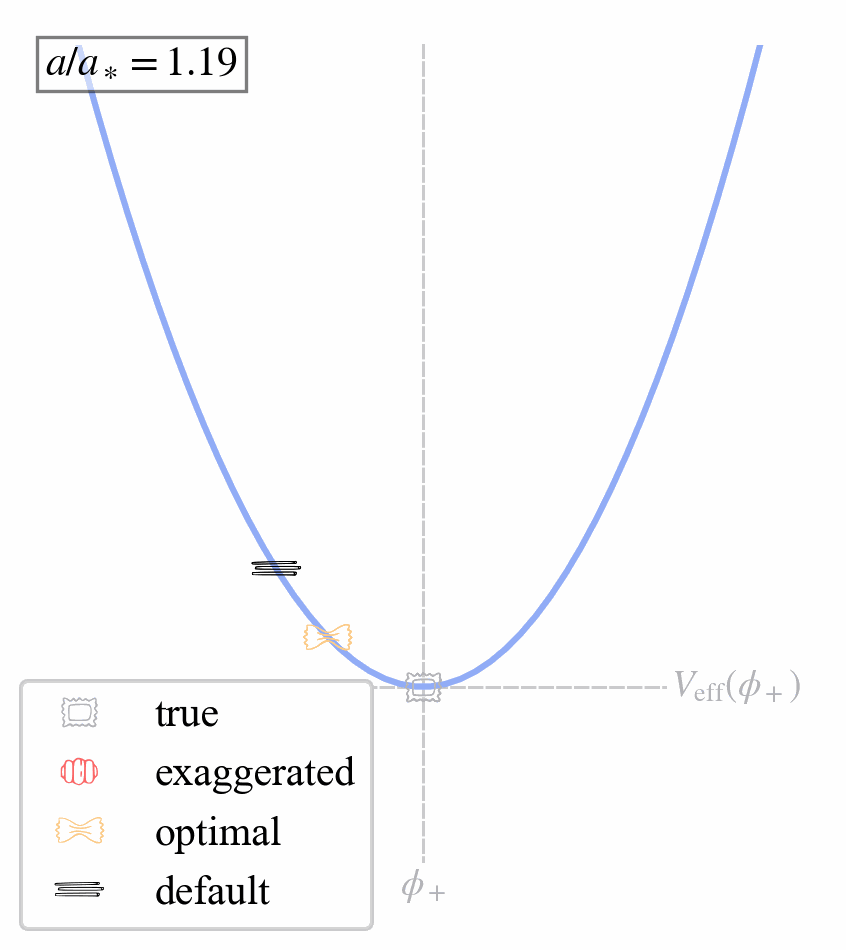
\includegraphics[keepaspectratio,width=\columnwidth,height=0.98\textheight]{gifs/asym_ball/asym_ball-199}
        \fi
        % ***********************
    \end{column}
    \end{columns}
    
% *************************************
% NOTES *******************************
\begin{notes}[1][animation]
    \nnote{1}{}
\end{notes}
% *************************************
\end{frame}


% \begin{frame}
%     \note{To clarify}
% \end{frame}